\chapter{Commande des robots manipulateurs I: quasi-statique}
\label{sec:staticcontrol}


Les objectifs en termes de mouvement désiré d'un robot sont généralement plus naturellement spécifiés en termes de variables dans l'espace de la tâche d'un robot, alors que à bas niveau les consignes des actionneurs sont reliés à des variables dans l'espace des joints. Ce chapitre présente des méthodes de commande qui permettent de calculer les consignes pour les actionneurs basé sur des objectifs directement spécifié dans l'espace de la tâche, malgré la relation géométrique hautement non-linéaire. Les méthodes ici présenté utilisent grandement les notions de cinématique différentiel et de statique présentés dans les sections \ref{sec:differentialkinematicmanipulators} et XXX.

Les méthodes présentés dans ce chapitre négligent les effets dynamiques (inerties, frottement, etc.) et considèrent juste un comportement simplifié des robots: la relation statique non-linéaire entre le mouvement/force des actionneurs et le mouvement/force à l'effecteur. Ces méthodes sont généralement performante lorsque les mouvements du robot sont relativement lents, c'est pourquoi ils sont ici regroupé sous la caractéristique "quasi-statique". Ensuite, selon la nature des actionneurs des systèmes robotiques, différentes variantes peuvent être utilisée:

\paragraph{Actionneurs commandés en vitesse:} Pour les méthodes de commande du mouvement de l'effecteur présentées aux sections \ref{sec:speedcontrol}, \ref{sec:positioncontrol} et \ref{sec:admcontrol}, il est considéré que le robot a des asservissements bas-niveau en vitesse à chacun des joints. Ces méthodes calculent les consignes en vitesse à envoyer aux joints pour contrôler le mouvement de l'effecteur. Ces méthodes fonctionnent bien dans des situations ou le suivi de consigne en vitesse des joints est très performant, c'est généralement le cas des manipulateurs industriels qui ont de très grand ratios de réduction. 

\paragraph{Actionneurs commandés en force:} Pour les méthodes de commande présentées aux section \ref{sec:forcecontrol} et \ref{sec:impcontrol}, on considère seulement la relation géométrique entre les forces des actionneurs et ceux à l'effecteur. Les deux méthodes calculent des forces à appliquer au niveau des actionneurs/joint, pour contrôler la force au niveau de l'effecteur. Ces méthodes fonctionnent donc bien pour des systèmes robotisées à basse impédance (peu d'inertie, peu d'effets dissipatifs, transmission réversibles, etc.), comme les systèmes haptiques où les forces des actionneurs sont pratiquement proportionnelles au courant dans les moteurs du à des très petits ratio de transmissions.



%%%%%%%%%%%%%%%%%%%%%%%%%%%%%%%%%%%%%%%%%%%%%%%%%%%%%%
\newpage
\section{Commande en vitesse de l'effecteur}
\label{sec:speedcontrol}
%%%%%%%%%%%%%%%%%%%%%%%%%%%%%%%%%%%%%%%%%%%%%%%%%%%%%%

Si un robot a des actionneurs contrôlés en vitesse à bas niveau, contrôler la vitesse de son effecteur se résume à mettre en oeuvre la relation de cinématique différentielle inverse (voir section \ref{sec:differentialkinematicmanipulators}).  Comme illustré par un schéma bloc à la Figure \ref{fig:robotspeedcontrol}, les consignes en vitesse pour les actionneurs sont déterminés en multipliant le vecteur-colonne de vitesses désirés dans l'espace des tâches, par l'inverse du Jacobien qui relie l'espace des joints à l'espace des tâches du systèmes. Le Jacobien est généralement dépendent de la position des joints du robot ce qui nécessite une boucle de rétroaction basé sur les capteurs de position des actionneurs pour effectuer le calcul de $J$ en continu basé sur la position actuel. Finalement, comme mis en évidence à la Figure \ref{fig:robotspeedcontrol}, cette méthode s'intègre comme une boucle haut-niveau pour coordonner les différents joints d'un système ou chacun des actionneurs est asservis en vitesse, souvent des boucles bas-niveaux implémentées directement dans l'électronique de contrôle des moteurs. 
%%%%%%%%%%%%%%%%%%%%%%%%%%%%%%%%
\begin{figure}[H]
	\centering
		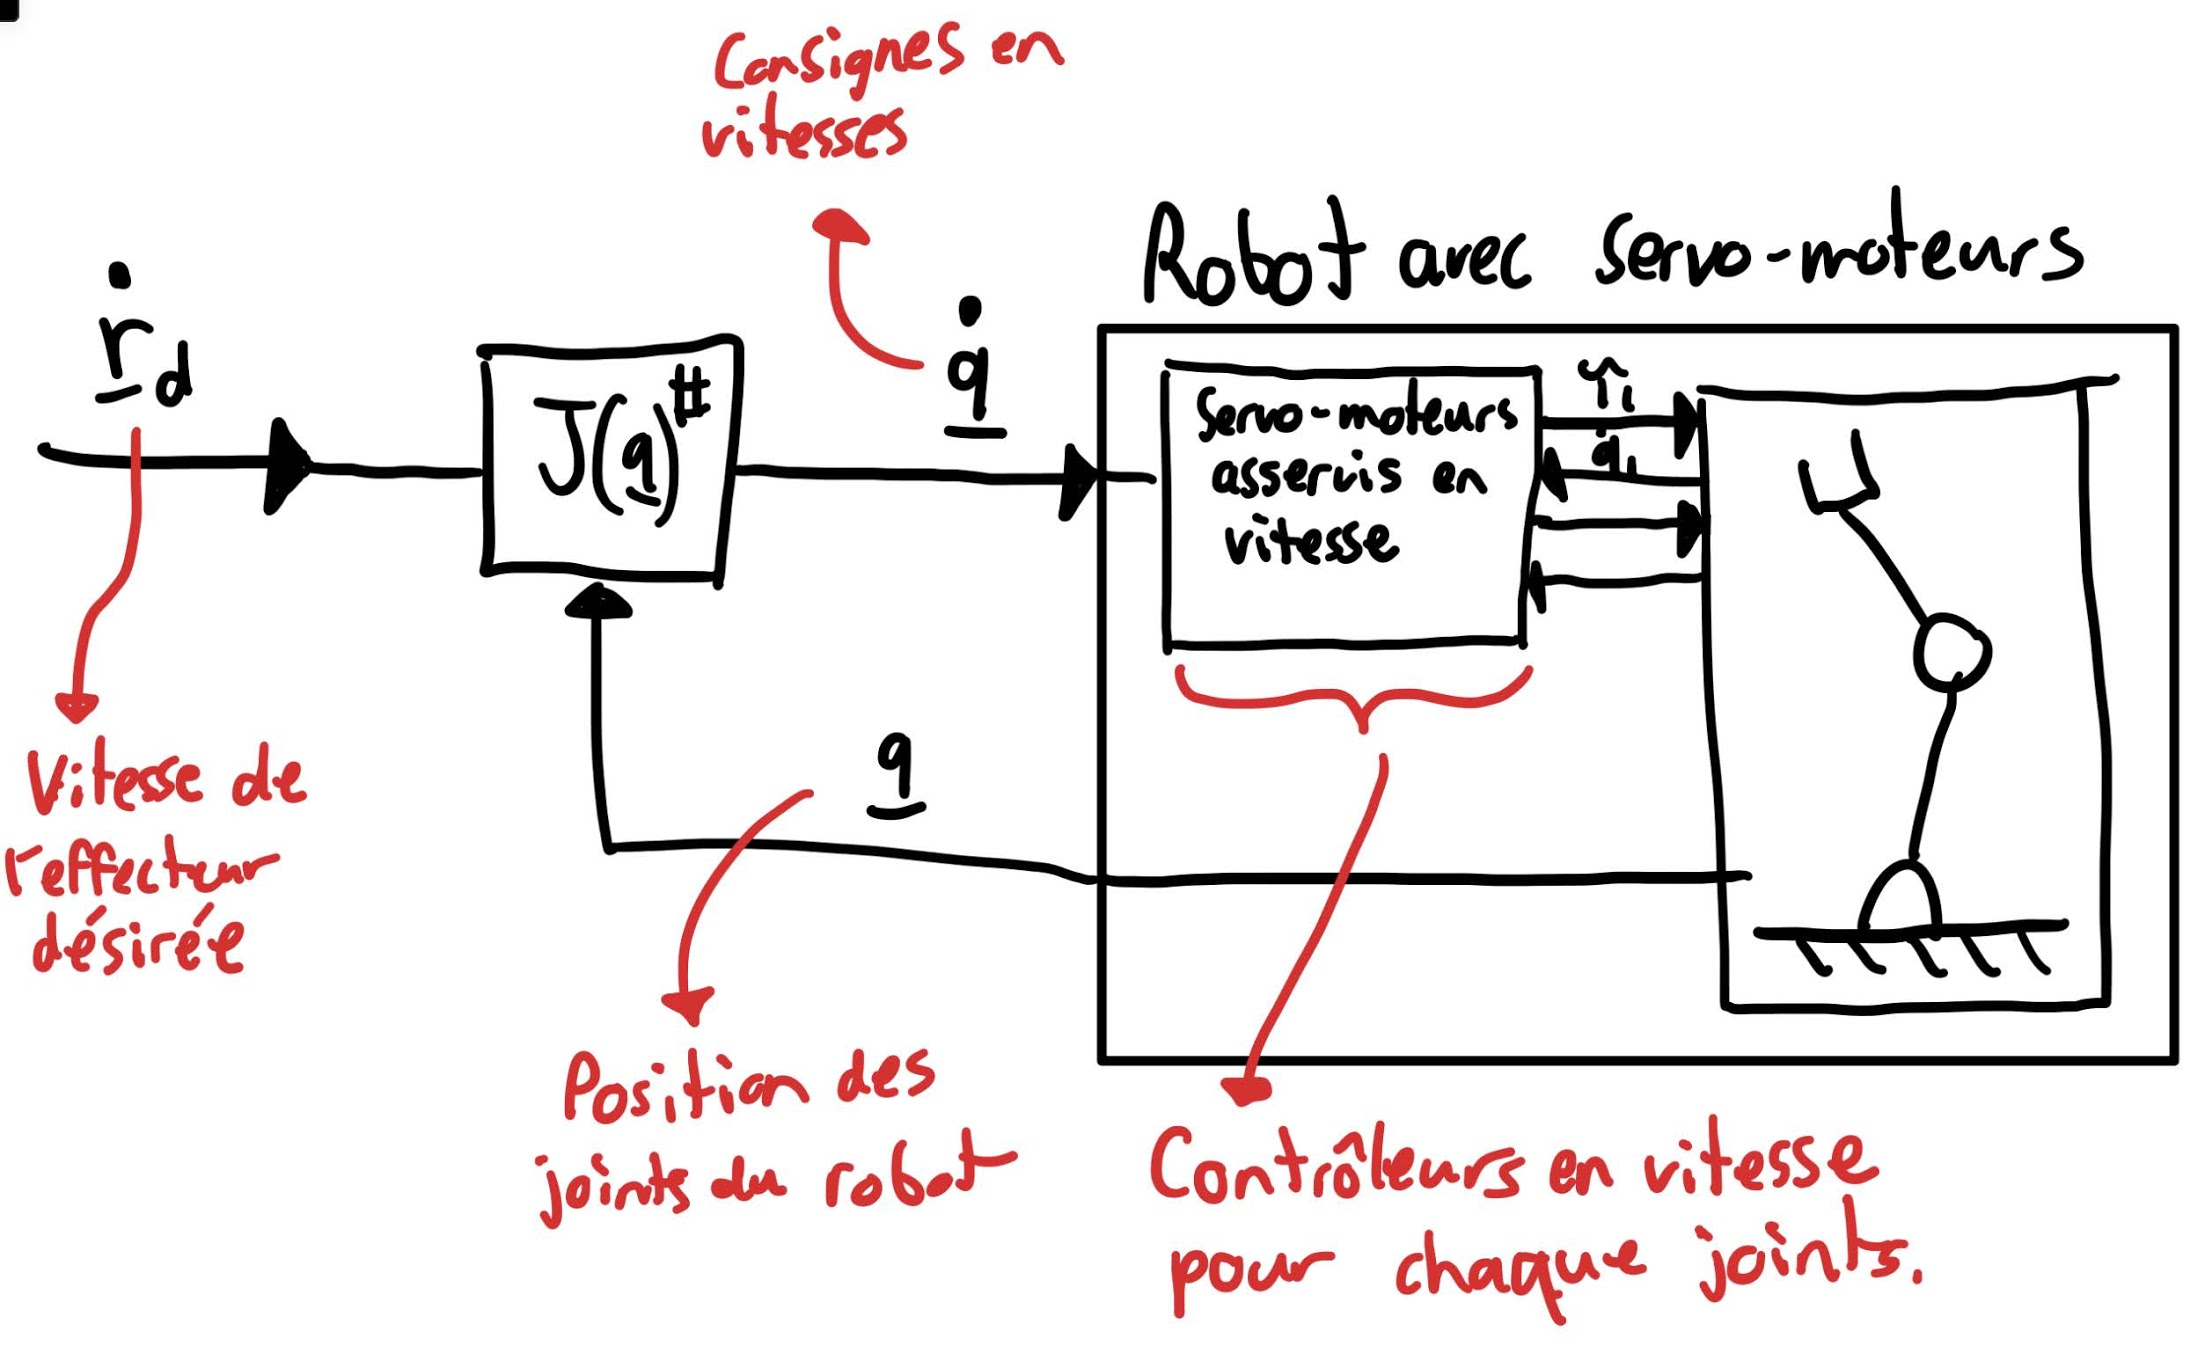
\includegraphics[width=0.7\textwidth]{fig/robotspeedcontrol.jpg}
	\caption{Commande de la vitesse de l'effecteur d'un robot : schéma bloc}
	\label{fig:robotspeedcontrol}
\end{figure}
%%%%%%%%%%%%%%%%%%%%%%%%%%%%%%%%

Si le nombre de joints $n$ est égale au nombre de DDL de l'espace de la tâche $m$, alors la matrice Jacobien est carrée et peut être inversée (sauf sur les singularités). Si le nombre de joint $n$ est supérieur au nombre de DDL de l'espace de la tâche $m$, alors on peut utiliser une matrice pseudo-inverse droite $J^{\#} = J^T (J J^T)^{-1}$ (voir section \label{sec:pseudoinverse}). La loi de commande en équation peut donc être exprimée comme:
%%%%%%%%%%%%%%%%%%
\begin{align}
\dot{\col{q}} = \left\{ \begin{array}{c}
 J(\col{q})^{-1} \dot{\col{r}_d}   \quad\quad \text{if $n=m$}
 \\ \\
 J(\col{q})^{\#} \, \dot{\col{r}_d}   \quad\quad \text{if $n>m$}
\end{array}
\right.
\end{align}
%%%%%%%%%%%%%%%%%

En substituant la loi de commande dans la relation de cinématique différentielle, on confirme que la vitesse de l'effecteur sera exactement la vitesse désirée:
%%%%%%%%%%%%%%%%%%
\begin{align}
\dot{\col{r}} &= J(\col{q}) \, \dot{\col{q}} \\
\dot{\col{r}} &= J(\col{q}) \, J(\col{q})^{\#} \, \dot{\col{r}_d} \\
\dot{\col{r}} &= J J^T (J J^T)^{-1} \, \dot{\col{r}_d} \\
\dot{\col{r}} &=  \dot{\col{r}_d} 
\end{align}
%%%%%%%%%%%%%%%%%
sous les hypothèses que: 1) le Jacobien utilisé par le contrôleur est exacte, 2) le Jacobien est inversible (i.e. le robot n'est pas sur une singularité) et 3) la vitesse des joints est parfaitement asservis par les boucles bas-niveaux. 




%%%%%%%%%%%%%%%%%%%%%%%%%%%%%%%%%%%%%%%%%%%%%%%%%%%%%%
\newpage
\section{Commande en position de l'effecteur}
\label{sec:positioncontrol}
%%%%%%%%%%%%%%%%%%%%%%%%%%%%%%%%%%%%%%%%%%%%%%%%%%%%%%

Pour commander la position de l'effecteur d'un robot, tenter de trouver une solution directement au problème de cinématique inverse (voir section \ref{sec:invkin} n'est généralement pas la méthode la plus appropriée car la cinématique directe des manipulateurs est hautement non-linéaire. La méthode ici présentée utilise plutôt la méthode de commande en vitesse de l'effecteur (section \ref{sec:speedcontrol}) pour indirectement résoudre la cinématique inverse du robot. L'idée ce résume à: si on peut contrôler la vitesse de l'effecteur de façon arbitraire, il suffit de diriger le vecteur vitesse de l'effecteur vers la position cible. La méthode est illustrée graphiquement à la Figure \ref{fig:robotspeedcontrolgeo}: 1) Un vecteur d'erreur $\col{r}_e$ est calculé en comparant la position désirée $\col{r}_d$ à la position actuelle $\col{r}$. 2) Le vecteur d'erreur $\col{r}_e$ est multiplié par un paramètre scalaire $\lambda$ pour déterminer la vitesse cible instantanée pour l'effecteur notée $\dot{\col{r}}_r$, qui point en direction de la cible. 3) L'inverse du Jacobien est utilisé pour convertir la vitesse instantanée désirée de l'effecteur en consigne de vitesse pour les joints. 
%%%%%%%%%%%%%%%%%%%%%%%%%%%%%%%%
\begin{figure}[H]
	\centering
		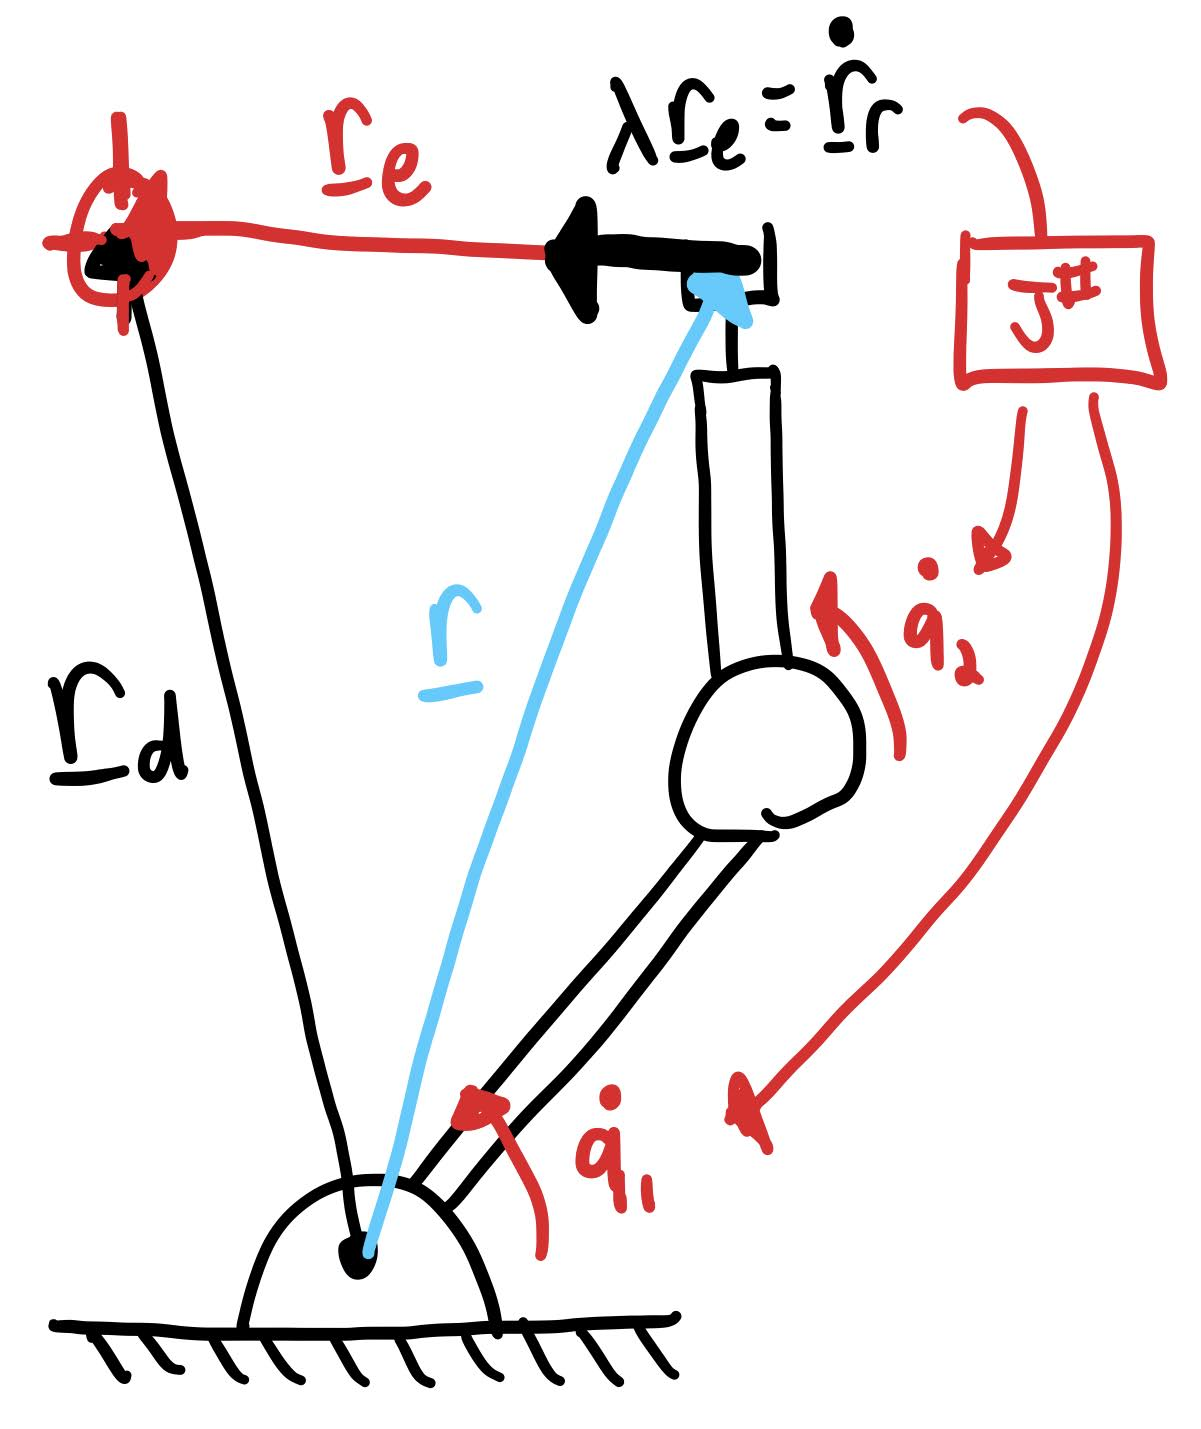
\includegraphics[width=0.4\textwidth]{fig/robotspeedcontrolgeo.jpg}
	\caption{Commande de la trajectoire de l'effecteur d'un robot : interprétation géométrique}
	\label{fig:robotspeedcontrolgeo}
\end{figure}
%%%%%%%%%%%%%%%%%%%%%%%%%%%%%%%%
Formellement, la loi de commande est exprimée par l'expression mathématique:
%%%%%%%%%%%%%%%%%%
\begin{align}
\dot{\col{q}} = \left\{ \begin{array}{c}
 J(\col{q})^{-1} \lambda 
 \underbrace{ \left( \col{r}_d  - \underbrace{f(\col{q})}_{\col{r}}  \right) }_{\col{r}_e} 
 \quad\quad \text{if $n=m$}
 \\ \\
 J(\col{q})^{\#} \, \lambda  \underbrace{ \left( \col{r}_d  - \underbrace{f(\col{q})}_{\col{r}}  \right) }_{\col{r}_e}    \quad\quad \text{if $n>m$}
\end{array}
\right.
\end{align}
%%%%%%%%%%%%%%%%%
ou $\lambda$ est un paramètre scalaire de gain du contrôleur, $J$ est le Jacobien, la matrice $n \times m$, qui relie l'espace des joints à l'espace de la tâche du manipulateur, et $f(\col{q})$ la fonction de cinématique directe du manipulateur. La Figure \ref{fig:robotspeedcontrolpos} illustre cette méthode de commande sous la forme d'un schéma bloc. 
%%%%%%%%%%%%%%%%%%%%%%%%%%%%%%%%
\begin{figure}[H]
	\centering
		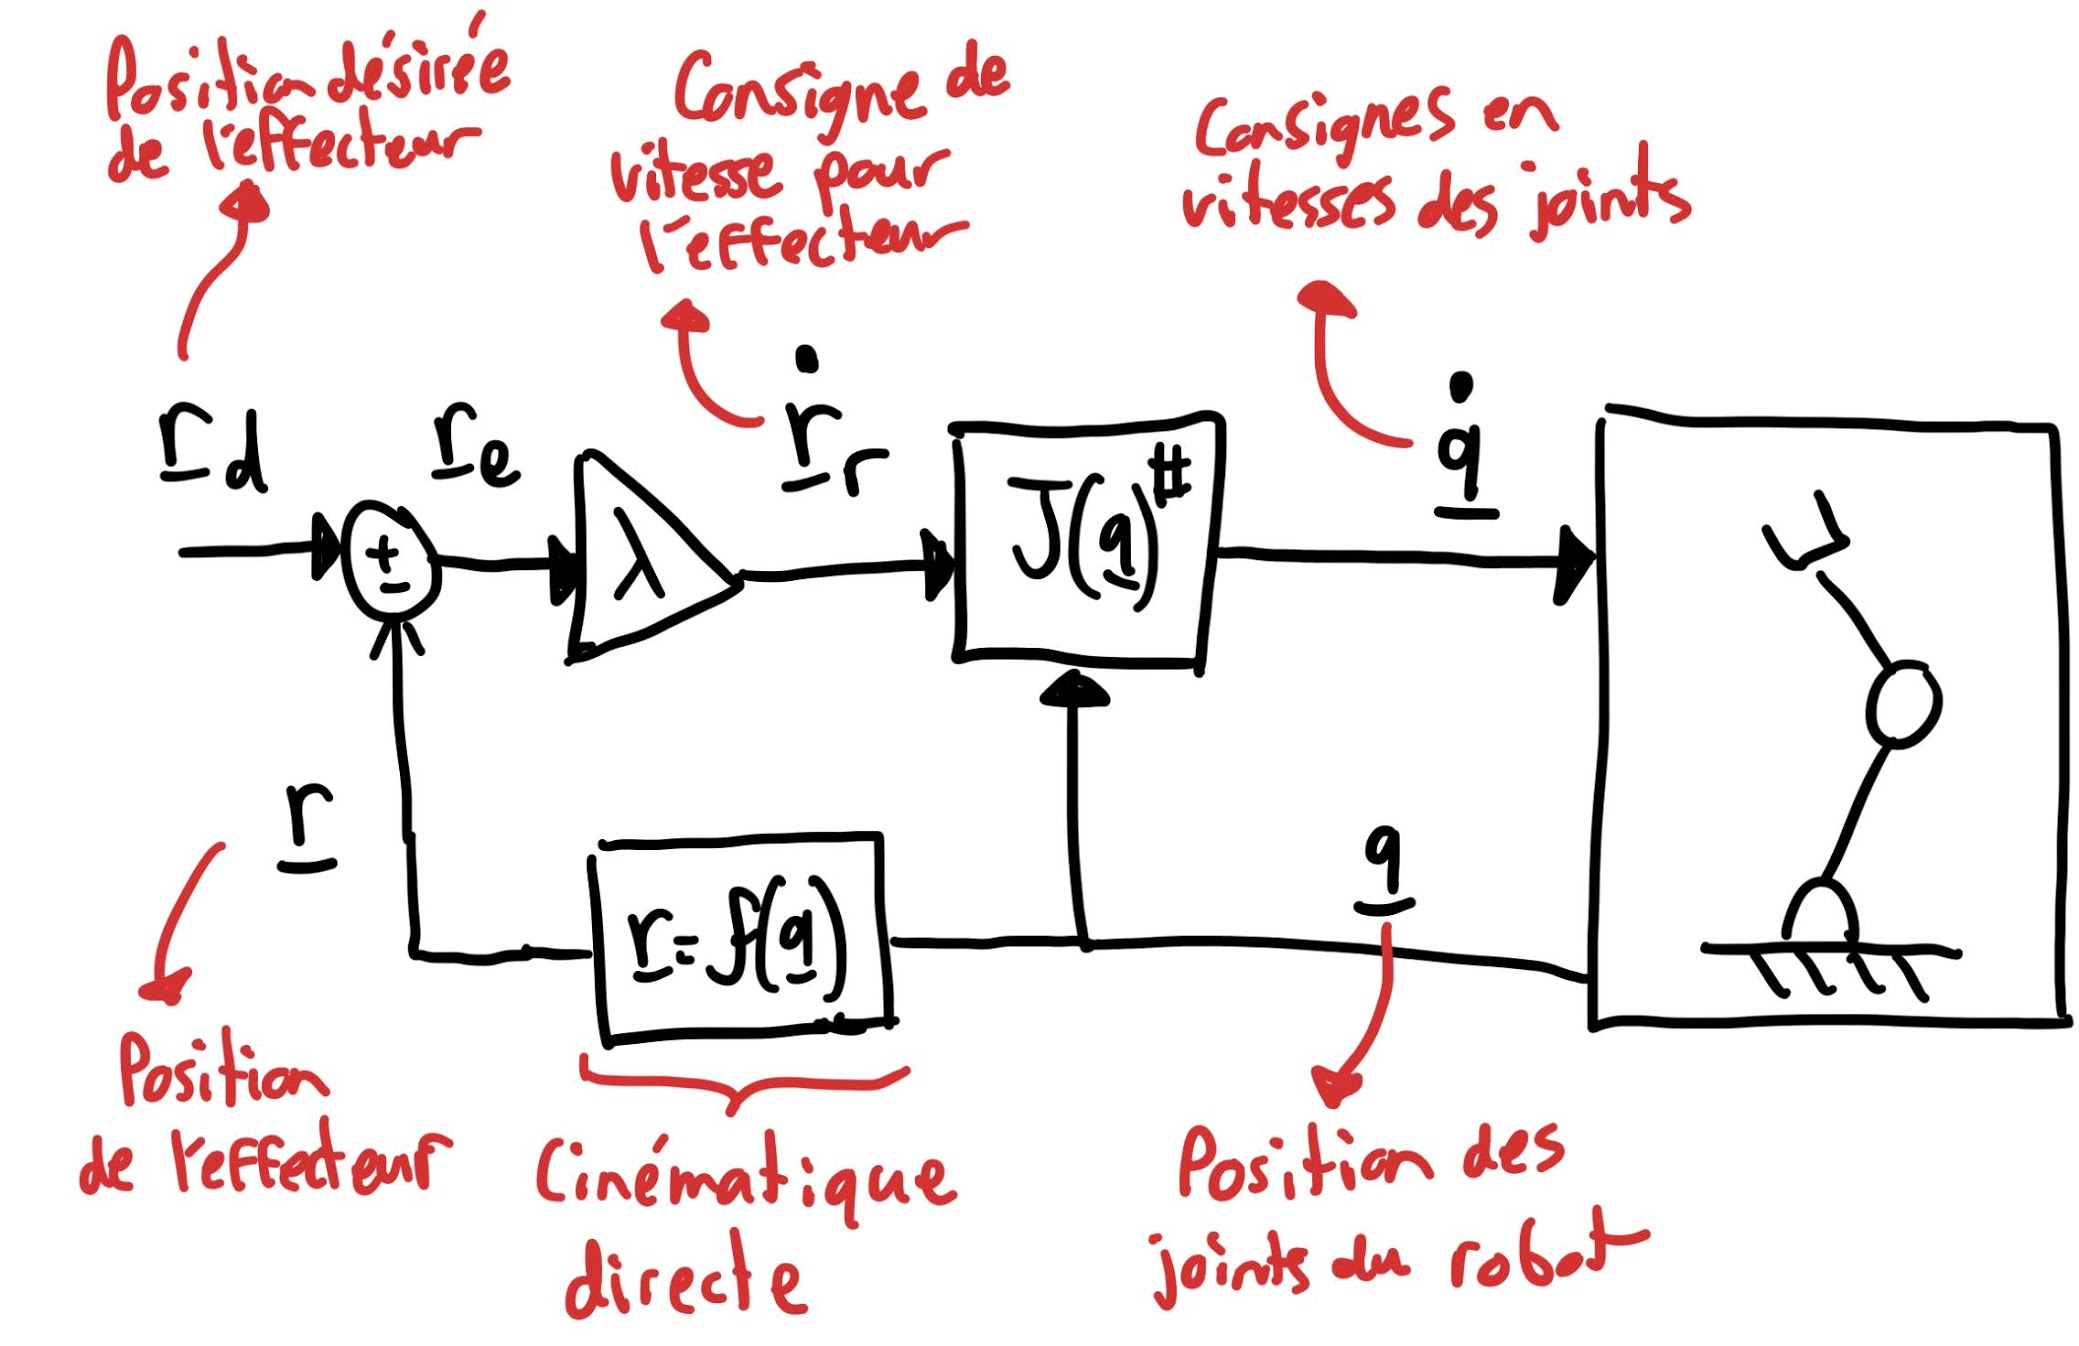
\includegraphics[width=0.7\textwidth]{fig/robotspeedcontrolpos.jpg}
	\caption{Commande de la position de l'effecteur d'un robot : schéma bloc}
	\label{fig:robotspeedcontrolpos}
\end{figure}
%%%%%%%%%%%%%%%%%%%%%%%%%%%%%%%%










%%%%%%%%%%%%%%%%%%%%%%%%%%%%%%%%%%%%%%%%%%%%%%%%%%%%%%%%%%%%%%%%
\subsection{Suivi de trajectoire}
\label{sec:trajcontrol}

Lorsque le robot doit suivre une position cible de l'effecteur qui varie dans le temps, il est préférable de calculer la dérivée temporelle de la trajectoire et d'utiliser cette information directement dans la loi de commande comme indiqué dans l'équation suivante:
%%%%%%%%%%%%%%%%%%
\begin{align}
\dot{\col{q}} = \left\{ \begin{array}{c}
 J(\col{q})^{-1} \left[ \dot{\col{r}_d} + \lambda \left( \col{r}_d  - \underbrace{f(\col{q})}_{\col{r}} \right) \right] \quad\quad \text{if $n=m$}
 \\ \\
 J(\col{q})^{\#} \, \left[ \dot{\col{r}_d} + \lambda \left( \col{r}_d  - \underbrace{f(\col{q})}_{\col{r}} \right) \right]   \quad\quad \text{if $n>m$}
\end{array}
\right.
\end{align}
%%%%%%%%%%%%%%%%%
En terme de schéma bloc, la vitesse de la trajectoire doit être utilisée avec un feedfoward dans la loi de commande comme illustré à la Figure \ref{fig:robotspeedcontroltraj}, pour garantir la convergence sur la trajectoire.
%%%%%%%%%%%%%%%%%%%%%%%%%%%%%%%%
\begin{figure}[H]
	\centering
		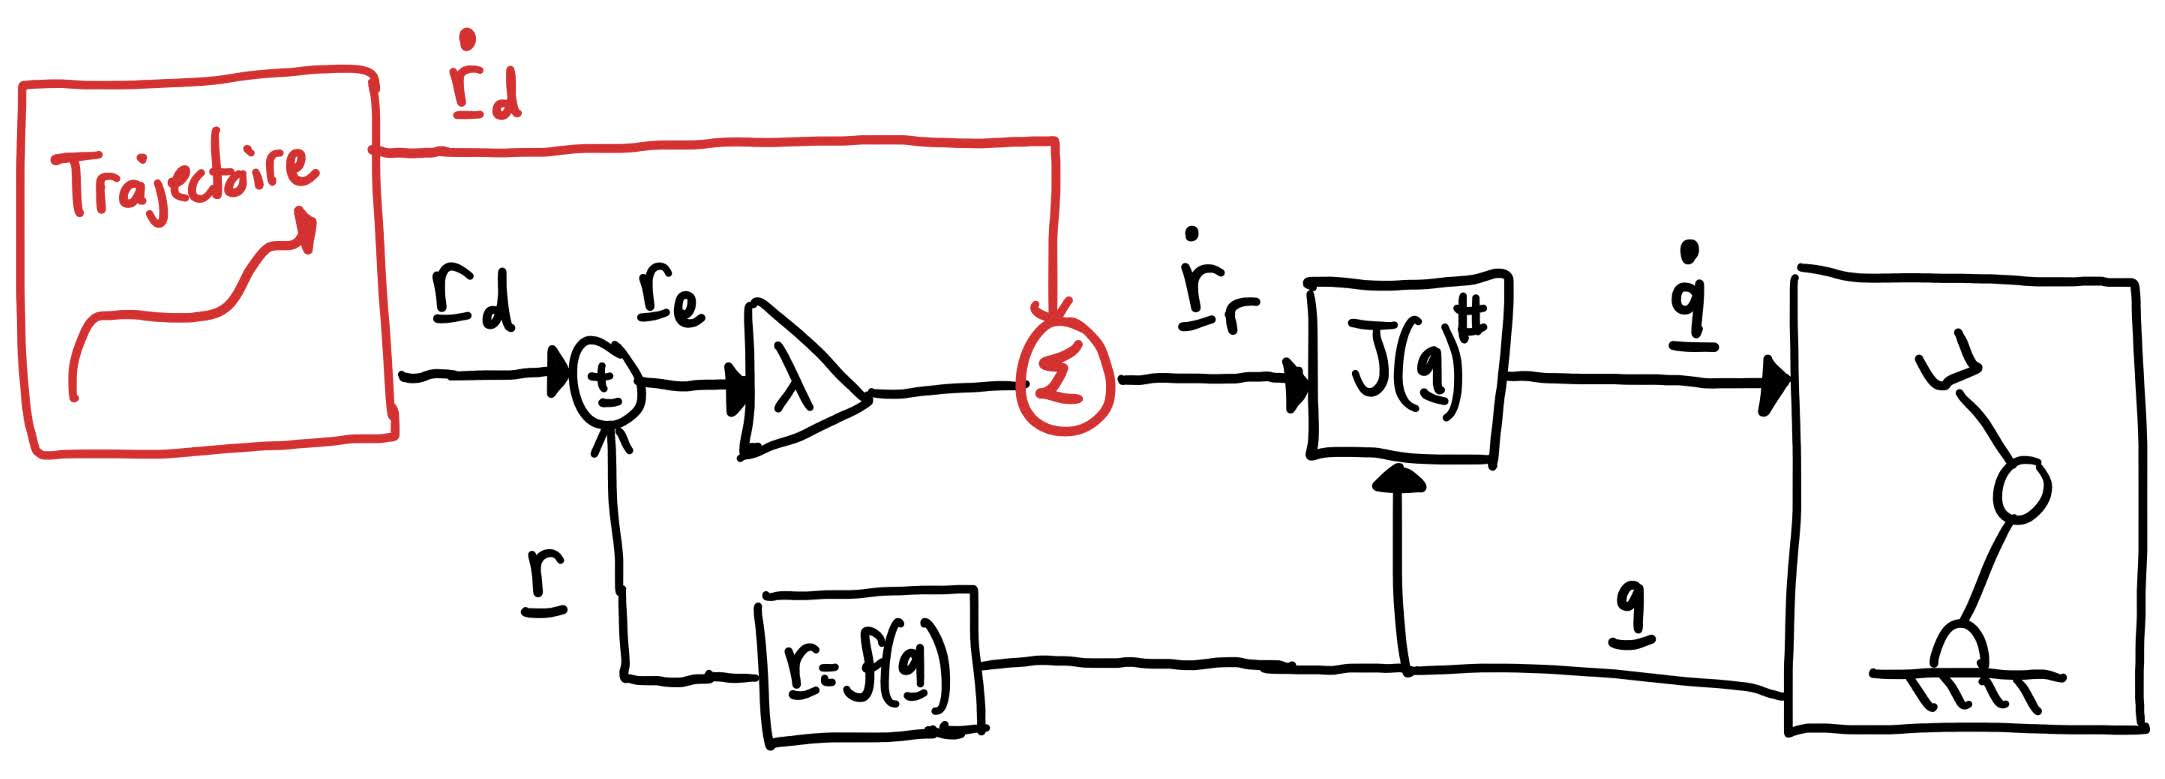
\includegraphics[width=0.95\textwidth]{fig/robotspeedcontroltraj.jpg}
	\caption{Commande de la trajectoire de l'effecteur d'un robot : schéma bloc}
	\label{fig:robotspeedcontroltraj}
\end{figure}
%%%%%%%%%%%%%%%%%%%%%%%%%%%%%%%%


\subsection{Convergence}

Les méthodes de commande en position de l'effecteur converge sous certaines conditions. L'objectif peut être mathématiquement exprimé comme:
%%%%%%%%%%%%%%%%%%
\begin{align}
\lim_{t \rightarrow \infty } \col{r}_e(t) = 0 
\end{align}
%%%%%%%%%%%%%%%%%
c'est-à-dire l'erreur (sur la position de l'effecteur) doit converger vers zéro. L'erreur est une fonction de la trajectoire et de la positon réelle du robot:
%%%%%%%%%%%%%%%%%%
\begin{align}
\col{r}_e = \col{r}_d - \col{r}
\end{align}
%%%%%%%%%%%%%%%%%
Si on dérive cette équation dans le temps, on obtient une relation différentielle. On peut alors substituer le modèle de cinématique différentiel et les lois de commandes pour obtenir:
%%%%%%%%%%%%%%%%%%
\begin{align}
\dot{\col{r}}_e 
&= \dot{\col{r}}_d - \dot{\col{r}} \\
&= \dot{\col{r}}_d - J(\col{q}) \dot{\col{q}} \\
&= \dot{\col{r}}_d - \underbrace{J(\col{q}) J(\col{q})^{\#} }_{1} \dot{\col{r}}_r \\
&= \dot{\col{r}}_d - \underbrace{J(\col{q}) J(\col{q})^{\#} }_{1}  \left( \dot{\col{r}}_d - \lambda \, \col{r}_e \right) \\
&= - \lambda \, \col{r}_e  
\end{align}
%%%%%%%%%%%%%%%%
La dynamique de l'erreur est donc stable et converge exponentiellement vers zéro si $\lambda>0$, avec une constante de temps égale à $\lambda$:
%%%%%%%%%%%%%%%%%%
\begin{align}
\dot{\col{r}}_e = - \lambda \, \col{r}_e 
\quad\quad \Rightarrow \quad\quad 
\col{r}_e(t) = \col{r}_e(t=0) \, e^{- \lambda t} 
\quad\quad \Rightarrow \quad\quad 
\col{r}_e(t=\infty) = 0
\end{align}
%%%%%%%%%%%%%%%%%
Notez ici que cette analyse assume un contrôle parfait et instantané de la vitesse des moteurs. Une autre limite est que la convergence cesse si le robot passe sur une singularité, i.e. mathématiquement l'inverse (ou pseudo-inverse) du Jacobien n'excisera pas. Aussi, comme démontrer dans la démarche, pour converger sur une trajectoire (position cible qui varie dans le temps), le feedforward illustré à la Figure \ref{fig:robotspeedcontroltraj} est nécessaire.


\subsection{Utilisation du Nullspace pour éviter les singularités}

À venir!

%%%%%%%%%%%%%%%%%%
\begin{align}
\dot{\col{q}} = J^{\#} \, \left[ \dot{\col{r}_d} + \lambda \left( \col{r}_d  - \underbrace{f(\col{q})}_{\col{r}}  \right)\right]  + \left[ I - J^{\#}J  \right] \col{v}
\end{align}
%%%%%%%%%%%%%%%%%



%%%%%%%%%%%%%%%%%%%%%%%%%%%%%%%%%%%%%%%%%%%%%%%%%%%%%%
\newpage
\section{Commande en force de l'effecteur}
\label{sec:forcecontrol}
%%%%%%%%%%%%%%%%%%%%%%%%%%%%%%%%%%%%%%%%%%%%%%%%%%%%%%





%%%%%%%%%%%%%%%%%%%%%%%%%%%%%%%%%%%%%%%%%%%%%%%%%%%%%%
\newpage
\section{Commande en impédance}
\label{sec:impcontrol}
%%%%%%%%%%%%%%%%%%%%%%%%%%%%%%%%%%%%%%%%%%%%%%%%%%%%%%


\subsection{Commande en impédance aux joints}
\label{sec:jointimpcontrol}

\subsection{Commande en impédance de l'effecteur}
\label{sec:effimpcontrol}



%%%%%%%%%%%%%%%%%%%%%%%%%%%%%%%%%%%%%%%%%%%%%%%%%%%%%%
\newpage
\section{Commande en admittance}
\label{sec:admcontrol}
%%%%%%%%%%%%%%%%%%%%%%%%%%%%%%%%%%%%%%%%%%%%%%%%%%%%%%



\subsection{Commande en admittance aux joints}
\label{sec:jointadmcontrol}

%%%%%%%%%%%%%%%%%%
\begin{align}
\dot{\col{q}} = Y(s) \col{\tau}_{c}
\end{align}
%%%%%%%%%%%%%%%%%

%%%%%%%%%%%%%%%%%%
\begin{align}
\dot{\col{q}} = Y(s) \col{\tau}_{c} = \left( M^{-1} \int + B^{-1}  + K^{-1} \frac{d}{dt}  \right) \col{\tau}_{c} \\
\col{q} = \frac{Y(s)}{s}  \col{\tau}_{c} = \left( M^{-1} \int \int + B^{-1} \int  + K^{-1}  \right) \col{\tau}_{c}
\end{align}
%%%%%%%%%%%%%%%%%

\subsection{Commande en admittance de l'effecteur}
\label{sec:effadmcontrol}

%%%%%%%%%%%%%%%%%%
\begin{align}
\dot{\col{q}} = \left\{ \begin{array}{c}
 J(\col{q})^{-1} \left( M^{-1} \int \col{f}_{c} + B^{-1} \col{f}_{c} + K^{-1} \frac{d}{dt} \col{f}_{c} \right)   \quad\quad \text{if $n=m$}
 \\ \\
 J(\col{q})^{\#} \, \left( M^{-1} \int \col{f}_{c} + B^{-1} \col{f}_{c} + K^{-1} \frac{d}{dt} \col{f}_{c} \right)  \quad\quad \text{if $n>m$}
\end{array}
\right.
\end{align}
%%%%%%%%%%%%%%%%%

